\section{Findings} % (fold)
\label{sec:findings}
With each approach we generate topics for the \crowdre{} dataset. In accordance with the predefined application domain labels, we expect to find four different topics: \textit{Energy, Entertainment, Health} and \textit{Safety}. Sentences labeled as \textit{Other} are assumed to be visible as noise in the result.
In our plots, we always plot the different requirement sentences. We use t-SNE to transform the embeddings into 2-dimensional space for our plots\,\cite{maaten_visualizing_2008}. The coloring is based on the application domain they were associated with and is as follows: \textcolor{clr_energy}{\emph{Energy}}, \textcolor{clr_entertainment}{\emph{Entertainment}}, \textcolor{clr_health}{\emph{Health}}, \textcolor{clr_safety}{\emph{Safety}} and \textcolor{clr_other}{\emph{Other}}.

\subsection{LDA} % (fold)
\label{sub:findings_lda}

Unfortunately, the result of the LDA doesn't match the expected topics. The approach itself creates some separable clusters, they can not be mapped to the expected ones considering the soft labeled domains. Still, some similarity between the requirements that are plotted next to each other can be found.

The processing time of the LDA approach is very fast which means the performance of is very good compared to approaches with high computational effort. The overall result for the LDA approach is that we couldn't gather the expected topics from the given dataset. 

\subsection{word2vec \& PCA} % (fold)
\label{sub:findings_w2v}
As shown in \autoref{fig:w2v-pretrained-4} we could identify two clusters using the word2vec. Again, this did not match our expected 4 clusters. Any interpretation of the plotted clusters may be only speculative and highly subjective, which is why we did not make any assumptions with regard to the data quality, yet.
Similar to the LDA, the performance was relatively good, though and we did not wait for our results for much longer than a couple of minutes.

\begin{figure}[ht]
  \begin{center}
    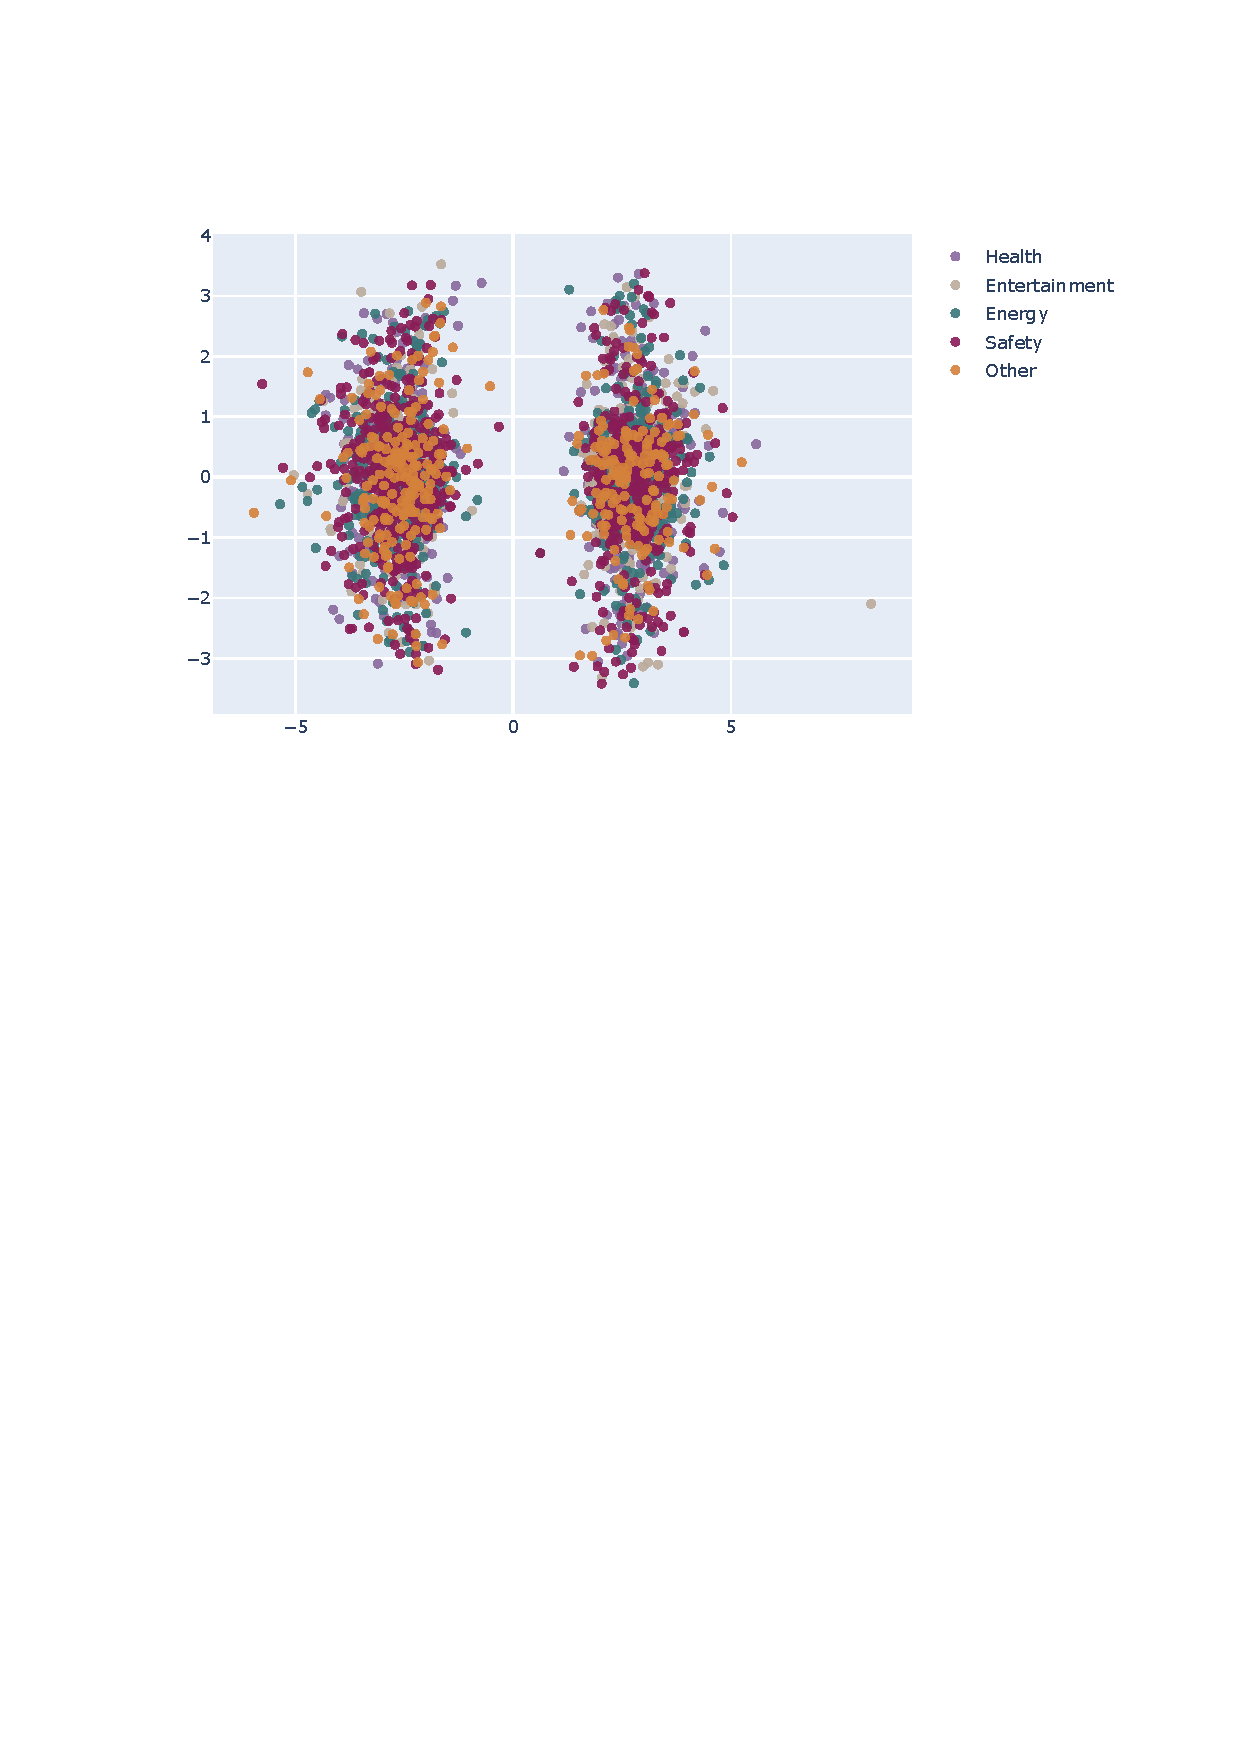
\includegraphics[width=\textwidth]{figures/word2vec_pretrained_pca-legend.pdf}
    \caption{word2vec result of the clustering using Google News word vectors}
    \label{fig:w2v-pretrained-4}
  \end{center}
\end{figure}
\FloatBarrier

\subsection{word2vec \& Word Mover's Distance} % (fold)
\label{sub:findings_wmd}
Using Word Mover's Distance, we achieve the best results, in the sense that we can not only distinguish clusters visually (see \autoref{fig:wmd-comparison}), but also by manual inspection of the sentence plotted next to each other.
When looking at the results in \autoref{fig:wmd-selftrained-1}, we can see that the domains \textit{Entertainment} (around the center) and \textit{Energy} (stretching from (0,-45) to (10,57)) can be well distinguished. Also, a cluster predominantly consisting of \textit{Health} sentences becomes apparent in the region from (0,20) to (70,45).
Judged by the pre-labeling only, it seems the clustering with our self-trained word vectors worked better. But manual inspection shows that the clustering based on the Google News vectors also brings new insights in the dataset. In \autoref{fig:wmd-pretrained-1} we can see, how the demarcation between the clusters is a lot clearer. Also, even though the sentences seem unrelated at first, the rightmost cluster (the area between (45,-15) and (75,30)) mostly contains sentences related parenting and children. Furthermore, the topmost cluster between (20,45) and (40,65) contains requirement sentences about animals. It becomes apparent, that the dataset may be clustered into different clusters than the 4 domain-based clusters we initially anticipated.\\

The higher quality of our results comes with a drawback of performance, though. On a current Intel i5-9600K 6-core processor with 3.7 GHz and 32 GB of memory attached, the calculation of the Word Mover's Distance matrix took approx. 45 minutes (even after splitting up the calculation to be done in 12 parallel threads and making use of the symmetry of the WMD).


\begin{figure}[hbt]
	\centering
	\subfigure[Self-trained word vectors\label{fig:wmd-selftrained-1}]{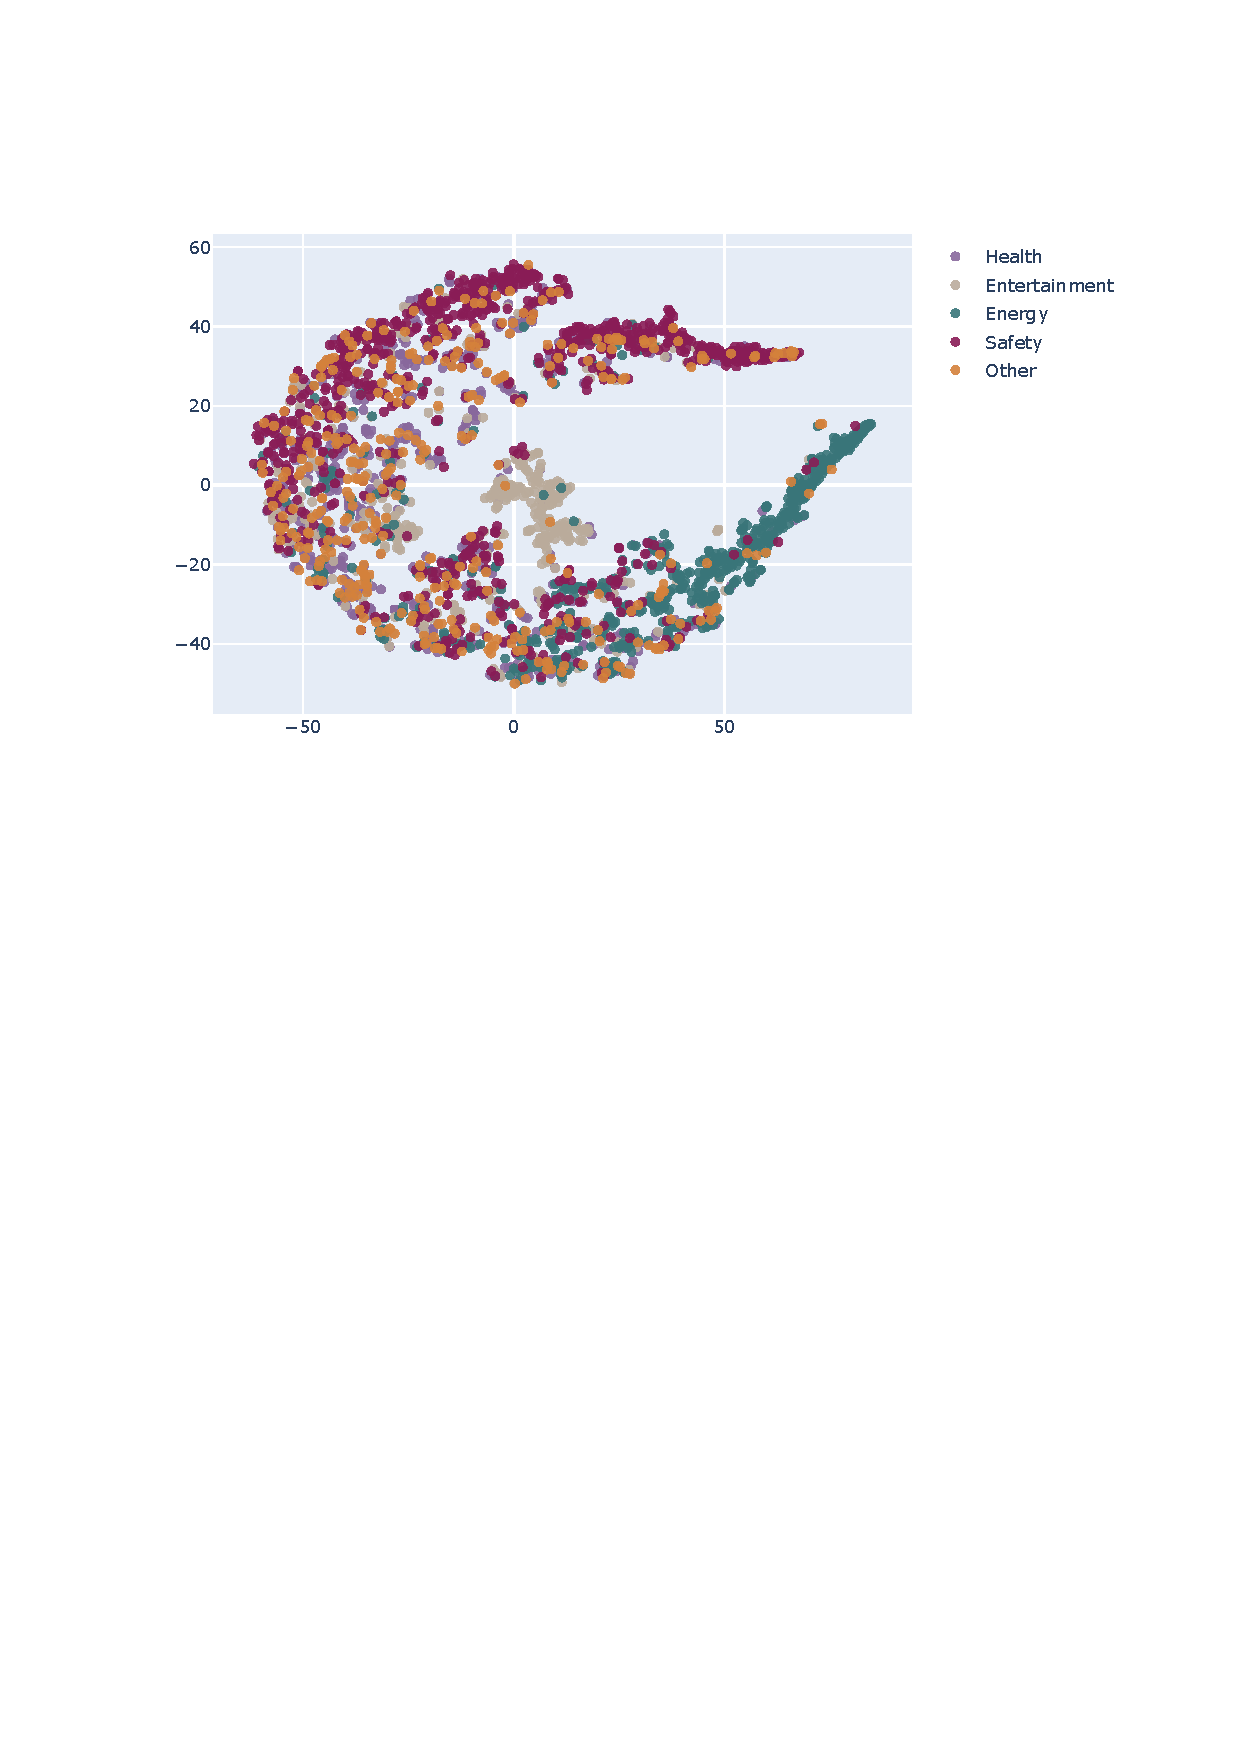
\includegraphics[width=0.49\textwidth]{figures/wmd_self_trained.pdf}}
    \subfigure[Google News word vectors\label{fig:wmd-pretrained-1}]{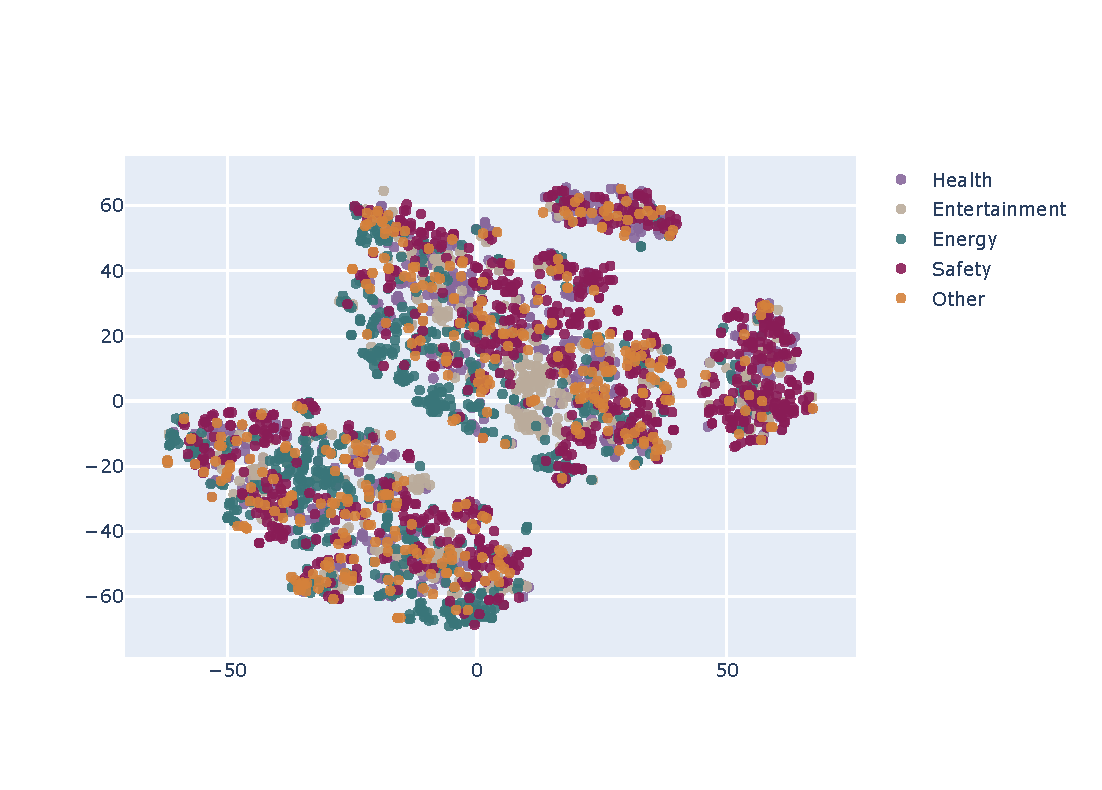
\includegraphics[width=0.49\textwidth]{figures/wmd_pretrained.pdf}}
    \caption{Results of the Word Mover's Distance}
    \label{fig:wmd-comparison}
\end{figure}
\FloatBarrier
% section analysis (end)